\documentclass[11pt]{article}

\usepackage{extras} % Se extras.sty



\begin{document}
\begin{titlepage}
\begin{center}

{\Large\bfseries TSEA56 - Kandidatprojekt i elektronik \\ LIPS Designspecifikation}

\vspace{5em}

Version 0.1

\vspace{5em}
Grupp 4 \\
\begin{tabular}{rl}
Hynén Ulfsjöö, Olle&\verb+ollul666+
\\
Wasteson, Emil&\verb+emiwa068+
\\
Tronje, Elena&\verb+eletr654+
\\
Gustafsson, Lovisa&\verb+lovgu777+
\\
Inge, Zimon&\verb+zimin415+
\\
Strömberg, Isak&\verb+isast763+
\\
\end{tabular}

\vspace{5em}
\today

\vspace{16em}
Status
\begin{longtable}{|l|l|l|} \hline

Granskad & - & - \\ \hline
Godkänd & - & - \\ \hline
 
\end{longtable}

\end{center}
\end{titlepage}

\pagebreak
\begin{center}

\section*{PROJEKTIDENTITET}
2016/VT, Undsättningsrobot Gr. 4

Linköpings tekniska högskola, ISY
\vspace{5em}
%\begin{center}

\begin{tabular}{|l|l|l|l|} \hline
\textbf{Namn} & \textbf{Ansvar} & \textbf{Telefon} & \textbf{E-post}  \\ \hline 
Isak Strömberg (IS) & Projektledare & 073-980 38 50 & isast763@student.liu.se \\ \hline
Olle Hynén Ulfsjöö (OHU)& Dokumentansvarig & 070-072 91 84 & ollul666@student.liu.se \\ \hline
Emil Wasteson (EW) & Hårdvaruansvarig & 076-836 61 66 & emiwa068@student.liu.se \\ \hline
Elena Tronje (ET) & Mjukvaruansvarig & 072-276 92 93 & eletr654@student.liu.se \\ \hline
Zimon Inge (ZI)& Testansvarig & 070-171 35 18 & zimin415@student.liu.se \\ \hline
Lovisa Gustafsson (LG) & Leveransansvarig & 070-210 32 53 & lovgu777@student.liu.se \\ \hline
\end{tabular}

%\end{center}

E-postlista för hela gruppen: isast763@student.liu.se

\vspace{5em}
Kund: ISY, Linköpings universitet 
tel: 013-28 10 00, fax: 013-13 92 82 \\
Kontaktperson hos kund: Mattias Krysander \\
tel: 013-28 21 98, e-post: matkr@isy.liu.se \\

\vspace{5em}
Kursansvarig:  Tomas Svensson\\
tel: 013-28 13 68, e-post: tomass@isy.liu.se \\
Handledare: Peter Johansson \\
tel: 013-28 13 45, e-post: peter.a.johansson@liu.se
\end{center}
\pagebreak

\tableofcontents

\pagebreak

\section*{Dokumenthistorik}
\begin{table}[h]
\begin{tabular}{|l|l|l|l|l|} \hline

\textbf{Version} & \textbf{Datum} & \textbf{Utförda förändringar} & \textbf{Utförda av} & \textbf{Granskad} \\ \hline
0.1 & - &  Första utkastet & Grupp 4 & - \\ \hline
\end{tabular}
\end{table}

\pagebreak
\pagenumbering{arabic}

\begin{flushleft}
\section{Inledning}
\lipsum

\subsection{Det totala systemet}
\lipsum


\subsection{Sensorer}
Roboten kommer vara utrustad med sex olika sensorer. Fyra infraröda sensorer av typen \verb+GP2D120+ används för att bestämma avstånden till väggarna på robotens sidor och robotens vinkel i förhållande till dessa, värden som anväds vid reglering av robotens rörelse rakt fram. Vidare finns ett kombinerat 3-axligt gyro och 3-axlig accelerometer av typen \verb+MPU-6500+ som används för att reglera rotation av roboten. Slutligen finns en lasersensor av typen \verb+Lidar-Lite v2+ för att bestämma avtåndet till väggar framför roboten. Placeringen av sensorerna visas nedan i figur \ref{sensor}.

\begin{figure}[htbp]
\centering
\noindent\resizebox{.8\linewidth}{!}{
	\documentclass[border=10px]{standalone}
\usepackage{tikz}
\usetikzlibrary{patterns}
\usetikzlibrary{shapes.arrows}
\usepackage{amssymb}
\usetikzlibrary{calc}
\usepackage{verbatim}
\begin{document}
	
\begin{tikzpicture}[scale=1,rotate=90]
		
	%Base
	\draw[thick, draw=black, fill=gray!10] (0,0) rectangle (6,10);

	%Wheels
	\draw[thick, pattern=north west lines, pattern color=black] (-.5,1) 		rectangle (0,2.5);
	\draw[thick, pattern=north west lines, pattern color=black] (-.5,7.5) 	rectangle (0,9);
	\draw[thick, pattern=north west lines, pattern color=black] (6,1) 		rectangle (6.5,2.5);
	\draw[thick, pattern=north west lines, pattern color=black] (6,7.5) 		rectangle (6.5,9);
	
	%Sensors
	\draw[thick, draw=black, fill=white] (-.25,.25) 		rectangle (.5,.75);
	\draw[thick, draw=black, fill=white] (-.25,9.25) 	rectangle (.5,9.75);
	\draw[thick, draw=black, fill=white] (5.5,.25) 		rectangle (6.25,.75);
	\draw[thick, draw=black, fill=white] (5.5,9.25) 		rectangle (6.25,9.75);
	\draw[thick, draw=black, fill=white] (2,10.25) 		rectangle (4,9.5);
	\draw[thick, draw=black, fill=white] (2.5,4) 		rectangle (3.5,6);
	
	%Arrows and text
	\draw[thick, ->]  (3,11) node[left, align=center] {\verb+LIDAR-Lite v2+ \\ + detektor av nödställd} -- (3,10.25);
	\draw[thick, <->] (0.5,0.5)  --  (5.5,0.5) node[left=-14pt,midway, fill=gray!10] {\verb+GP2D120+};
	\draw[thick, <->] (0.5,9.5) -- (3,9) node[right=-14pt,fill=gray!10] {\verb+GP2D120+} -- (5.5,9.5);
	\draw[thick, ->] (4.5,5) node[above] {\verb+MLX90609+} -- (3.5,5);
	\end{tikzpicture}
	
\end{document}}
	\caption{Placering av sensorer \label{sensor}}	
\end{figure}

\subsection{Ställdon}
Roboten kommer använda sig av totalt sex olika ställdon. Fyra av dessa är motorerna som driver varsitt hjul. Motorerna kan dock inte styras individuellt utan enbart parvis, varför de egentligen kan ses som två enheter. Utöver dessa ska roboten ha ett servo i gripklon, för att kunna öppna och stänga densamma, och ett servo för rotation av lasersensorn.
\begin{figure}[htbp]
\centering
\noindent\resizebox{.8\linewidth}{!}{
	\documentclass[border=10px]{standalone}
\usepackage{tikz}
\usetikzlibrary{patterns}
\usetikzlibrary{shapes.arrows}
\usepackage{amssymb}
\usetikzlibrary{calc}
\usepackage{verbatim}
\begin{document}
	
\begin{tikzpicture}[scale=1,rotate=90]
		
	%Base
	\draw[thick, draw=black, fill=gray!10] (0,0) rectangle (6,10);

	%Wheels
	\draw[thick, pattern=north west lines, pattern color=black] (-.5,1) 		rectangle (0,2.5);
	\draw[thick, pattern=north west lines, pattern color=black] (-.5,7.5) 	rectangle (0,9);
	\draw[thick, pattern=north west lines, pattern color=black] (6,1) 		rectangle (6.5,2.5);
	\draw[thick, pattern=north west lines, pattern color=black] (6,7.5) 		rectangle (6.5,9);
	
	%Motors
	\draw[thick, draw=black, fill=white] (.25,1.1) 		rectangle (1.5,2.4);
	\draw[thick, draw=black, fill=white] (.25,7.6) 	rectangle (1.5,8.9);
	\draw[thick, draw=black, fill=white] (4.5,1.1) 		rectangle (5.75,2.4);
	\draw[thick, draw=black, fill=white] (4.5,7.6) 		rectangle (5.75,8.9);
	
	%Servos
	\draw[thick, draw=black, fill=white] (2,9.5) 		rectangle (3,8.5);
	\draw[thick, draw=black, fill=white] (3,9.5) 		rectangle (4,8.5);
	
	%Arrows and text
	\draw[thick, ->]  (3.5,11) node[left, align=center] {Servo för laser} -- (3.5,10.25);
	\draw[thick, <->] (1,1.75)  --  (3,7) -- (5,1.75);
	\draw[thick, <->] (1,8.25) -- (3,7) node[right=-14pt,fill=gray!10] {Motorer} -- (5,8.25);
	\draw[thick, ->] (2.5,11) node[left] {Servo för gripklo} -- (2.5,10.25);
	\end{tikzpicture}
	
\end{document}}
	\caption{Placering av ställdon \label{ställdon}}	
\end{figure}

\pagebreak
\section{Delmodul 1 - Huvudmodul}
\lipsum

\subsection{Detaljerad beskrivning}
\lipsum

\subsection{Hårdvara}
\lipsum

\subsection{Mjukvara}
\lipsum

\pagebreak
\section{Delmodul 2 - Sensormodul}
Sensormodulens uppdrag är att kommunicera med både sensorerna och huvudmodulen. Mätdata samplas med konstant frekvens och konverteras därefter till motsvarande SI-enhet. För avståndssensorerna innebär detta att den analoga inspänningen konverteras till ett digitalt värde i enheten meter.

Den främre avståndssensorn (laser-sensorn) placeras på ett roterande servo så att den kan \emph{scanna} korridoren roboten befinner sig i. Detta förutsätter att servot går att styra så att vinkelutslaget går att beräkna med godtycklig precision. Tillåter inte servot en sådan styrning placeras laser-sensorn så att den konstant pekar rakt framåt.

Vinkelhastighets-sensorerna används för att beräkna vinkelutslag då roboten tar en sväng. Mätdatan behöver därför integreras under ett tidsintervall och konverteras till en vinkel. Hur den nödställde ska representeras är ännu inte fastställt. Förslagsvis används en IR-fyr i kombination med en IR-sensor. Sensormodulens uppdrag blir då att ta beslutet om när den nödställde är funnen.

\subsection{Detaljerad beskrivning}
\lipsum

\subsection{Hårdvara}
De sensorer som används är följande,



\subsubsection{IR-sensor, GP2D120}
	\item[Avstånd] \hfill \\

\subsubsection{Laser-sensor, LIDAR-Lite v2}
Lidar-Lite v2 är en kraftfull lasersensor av begränsad storlek med ett flertal funktioner ändamålsenliga för exempelvis en undsätnningsrobot. Utöver att kunna möta avstånd, så kan den dessutom mäta hastighet och signalstyrka hos mål på upptill 40 meters avstånd. Detta med en felmarginal på 0,025 meter. Andra fördelar hos sensorn inkluderar låg strömkonsumtion och en upplösning 0,01 meter \cite{7131685}.

Kommunikationen mellan Lidar-Lite v2 och microprocessorn, Atmega16, kommer att ske via ett PWM-interface som lasersensorn kommer med i sitt grundutförande. 


\subsubsection{Gyro/accelerometer, MPU-6500}
\item[Vinkelhastighet] \hfill \\
 
\subsubsection{IR-detektor, IRM-8601-S}
\item[Identifierare av nödställd] \hfill \\
	

\subsection{Mjukvara}
\lipsum

\pagebreak
\section{Delmodul 3 - Styrmodul}
Styrmodulens uppgift är att översätta styrkommandon till servostyrning av de fyra hjulen och gripklon. Styrkommandona kommer via en I\textsuperscript{2}C-bussen från huvudmodulen och konverteras därefter till en PWM-sekvens. PWM-sekvensen skickas till gripklon respektive H-bryggorna som styr ett hjulpar var. 

Kopplingsschemat ser ut enligt figur \ref{kopplingsschema:styrmodul}, det framgår från figuren att utgångarna från \verb+ATmega16+ räcker för modulens ändamål. Både avbrottsingång \verb+INT0+ och \verb+INT1+ används inte men reservas ifall ytterligare funktionalitet önskas lägga till. Det finns även möjlighet att att styra en extra komponent via PWM eftersom utgången \verb+OC2+ är oanvänd.  

Prestandan hos \verb+ATmega+ räcker för modulens syfte. 
 
\subsection{Detaljerad beskrivning}
Nedan följer en beskrivning av vilka styrkommandon styrmodulen ska kunna ta emot, hur kommunikationsprotokollet ser ut, hur regleringen ska ske samt lite övrig fakta kring modulen.

\subsubsection{Styrkommandon}\label{Styrkommandon}
Styrmodulen tar emot kommandon från huvudmodulen och verkställer dessa. Följande kommandon kommer kunna skickas: \textit{reglering av/på, gripklo öppna/stäng, fram/bak, sväng höger/vänster, rotera höger/vänster och stopp}. Kommandot \textit{reglering av/på} ställer in styrmodulen för manuell eller autonom körning, vilket påverkar tolkningen av det data som skickas från huvudmodulen.

Tillsammans med kommandona för rörelse skickas även ett tal som, beroende på om reglering är aktiverad eller inte, anger en sträcka/vinkel för förflyttningen eller med vilken hastighet (i procent av maxhastighet) förflyttningen ska utföras. Ett kommando kan exempelvis se ut såhär: \textit{fram 80}, varpå roboten antingen kör framåt 80 cm eller med 80\% av maxhastighet, beroende på om regleringen är aktiverad eller inte. Modulen kommer vara designad så att ett körkommando gäller tills dess att ett nytt kommando skickas, varför även kommandot för \textit{stopp} är nödvändigt.

Eftersom kommandona till styrmodulen skickas på den form som visats ovan kommer all reglering behöva ske i styrmodulen. Därför kommer även mätdata att tas emot från huvudmodulen. Beroende på vilken typ av förflyttning roboten utför så kommer följande sensorvärden att skickas från huvudmodulen:
\begin{itemize}
	\item fram/bak - avstånd till vägg fram och på sidorna.
	\item sväng höger/vänster - inga (kommandot används enbart vid manuell styrning och behöver således inte regleras).
	\item rotera höger/vänster - vinkel och vinkelhastighet.
\end{itemize}
Dessa sensorvärden kommer skickas med en frekvens av \textcolor{red}{x} Hz förutsatt att reglering är aktiverad, dvs vid autonom styrning av roboten.

\subsubsection{Kommunikationsprotokoll}
Följande protokoll används för att skicka data till styrmodulen:
\begin{figure}[htbp]
\centering
\noindent\resizebox{.8\linewidth}{!}{
	\documentclass[crop,tikz]{standalone}
\usepackage{tikz}
\usetikzlibrary{calc}
\usetikzlibrary{positioning}
\begin{document}
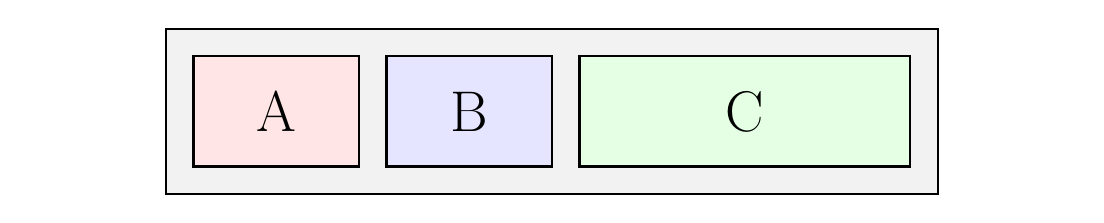
\begin{tikzpicture}[scale=0.07,rotate=0]
	
	%Background
	\draw[draw=white, fill=white] (0,0) rectangle (190,30);
		
	%Frame
	\draw[thick, draw=black, fill=gray!10] (25,0) rectangle (165,30);

	%Segments
	%A
	\draw[thick, draw=black, fill=red!10] (30,5) rectangle (60,25);
	\node at (45,15) {\huge A};

	%B
	\draw[thick, draw=black, fill=blue!10] (65,5) rectangle (95,25);
	\node at (80,15) {\huge B};
	
	%C
	\draw[thick, draw=black, fill=green!10] (100,5) rectangle (160,25);
	\node at (130,15) {\huge C};
	

	
\end{tikzpicture}
\end{document}}
	\caption{Protokoll för dataöverföring mellan huvud- och styrenhet\label{styrdata}}	
\end{figure}

Där respektive segment motsvarar följande: 
\begin{itemize}
	\item A (Bit x-y) - Startbit
	\item B (Bit x-y) - Definierar om ett körkommando eller ett sensorvärde skickas.
	\item C (Bit x-y) - Definierar vilket kommando eller vilken typ av värde som skickas.
	\item D (Bit x-y) - Hastighet (om körkommando och inte reglering), sträcka/vinkel (om körkommande och reglering) eller värde (om sensorvärde).
	\item E (Bit x-y) - Slutbit
\end{itemize}

\subsubsection{Reglering}
Vid manuell styrning av roboten sker ingen reglering. Detta för att användaren ska få ohämmad kontroll över roboten och förväntas sköta ``regleringen'' manuellt. Vid autonom styrning kommer dock alla förflyttningar behöva regleras. Som nämnt i avsnitt \ref{Styrkommandon} kommer huvudmodulen skicka relevanta sensorvärden vid autonom körning. Beroende på vilket styrkommando som skickats väljer styrmodulen sedan en styrmod och reglerar rörelsen. De olika styrmoderna och hur deras reglering sker finns beskrivet mer ingående i Appendix \textcolor{red}{x}.

\subsubsection{Övrigt}
Plattformen som roboten byggs på har färdiga kretsar för att styra chassits hjul. Hjulen kan styras parvis (höger och vänster) genom att sätta en bit för att bestämma rotationsriktningen och sedan skicka en PWM-signal för att bestämma rotationshastigheten. Roboten styrs alltså differentiellt, dvs genom olika hastighet på höger och vänster sida.

Roboten ska även vara utrustad med en gripklo, för att kunna greppa de förnödenheter som ka transporteras. Klons aktiva del består av ett servo av typen \verb+RG-180+ som styrs med en PWM-signal.

Det ska även finnas en alphanumerisk LCD-display, av typen \verb+LCD JM162A+, på roboten, som används för att visa relevanta sensorvärden vid reglering. Den har totalt 16 pinnar, varav åtta är databitar, tre används för konfiguration och resterane är referensignaler och strömtillförsel.

\subsection{Hårdvara}
Styrmodulen kommer kräva följande hårdvara:
\begin{itemize}
	\item ATmega16
	\item Robotplattform (Terminator)
	\item Gripklo %Specificera senare
\end{itemize}

\subsection{Mjukvara}
Koden för styrmodulen är skriven i C och består främst av två delar, reglering och display. Gripklon styrs direkt av ett styrkommando och kan endast öppnas respektive stängas.

\subsubsection{Display}
Displayen är en alphanumerisk 16x2 LCD-display och ska visa utvalda sensorvärden i realtid. I koden används drivrutinen \emph{lcd.h} för att initiera och skriva text till displayen. Genom att anropa initieringsmetoden rensas displayen och pekaren placeras på rätt position. Därefter skrivs typen av mätvärde och det faktiska värdet ut. Tack vare två rader kan flera mätvärden skrivas ut samtidigt, förslagsvis ett i respektive hörn av displayen.

Utskriften till displayen sker i huvudloopen och i takt med att nya mätvärden tas emot.

\subsubsection{Reglering}
När styrmodulen tar emot ett kommando från huvudmodulen så regleras servona utifrån de senaste mottagna sensorvärdena. Den reglering som programmeras till modulen består av tre komponenter. Den ena ser till att roboten färdas i mitten av korridoren, den andra anpassar hastigheten utifrån korridorens längd och den tredje ser till att en sväng tas vinkelrätt.

Isak: fortsätt på stycket och förklara regleringen utifrån din förstudie




\pagebreak
\section{Delmodul 4 - Datormodul}
\lipsum

\subsection{Detaljerad beskrivning}
\lipsum

\subsection{Hårdvara}
Datormodulen kräver en dator kompatibel med Java.

\subsection{Mjukvara}
\lipsum

\pagebreak
\section{Intermodulär kommunikation}
\lipsum

\subsection{I\textsuperscript{2}C-buss}
\lipsum

\subsection{Bluetooth\textsuperscript{\circledR}-kommunikation}
\lipsum

\pagebreak
\section{Implementering}
\lipsum

\pagebreak
\addcontentsline{toc}{section}{Referenser}
\bibliographystyle{ieeetr}
\bibliography{references}

\end{flushleft}

\end{document}